\section{data}\label{sec:data}
Molino (15,000 Mocks): 
$\Omega_{Μ}$=0.32, $\sigma$8=0.834,  Volume ~ 1 Gpc/h3 
Galaxy catalogs from the Quijote N-body simulations (Villaescusa-Navarro et al.2020) with the standard Halo Occupation Distribution model from Zheng et al. (2007). HOD parameters are based on high luminosity SDSS samples. More at changhoonhahn.github.io/molino

And two other series of mocks provided by our DESI collaborators:
GLAM (1,000 Mocks)

Abacus (25 mocks)


Fig. \ref{fig:data} shows the mean bispectrum (left) and the mean power spectrum (right) for the GLAM and ABACUS simulations, relative to the spectra without the BAO signal, which is simulation-based for the GLAM realizations and theory-based for the ABACUS.

\begin{figure*}
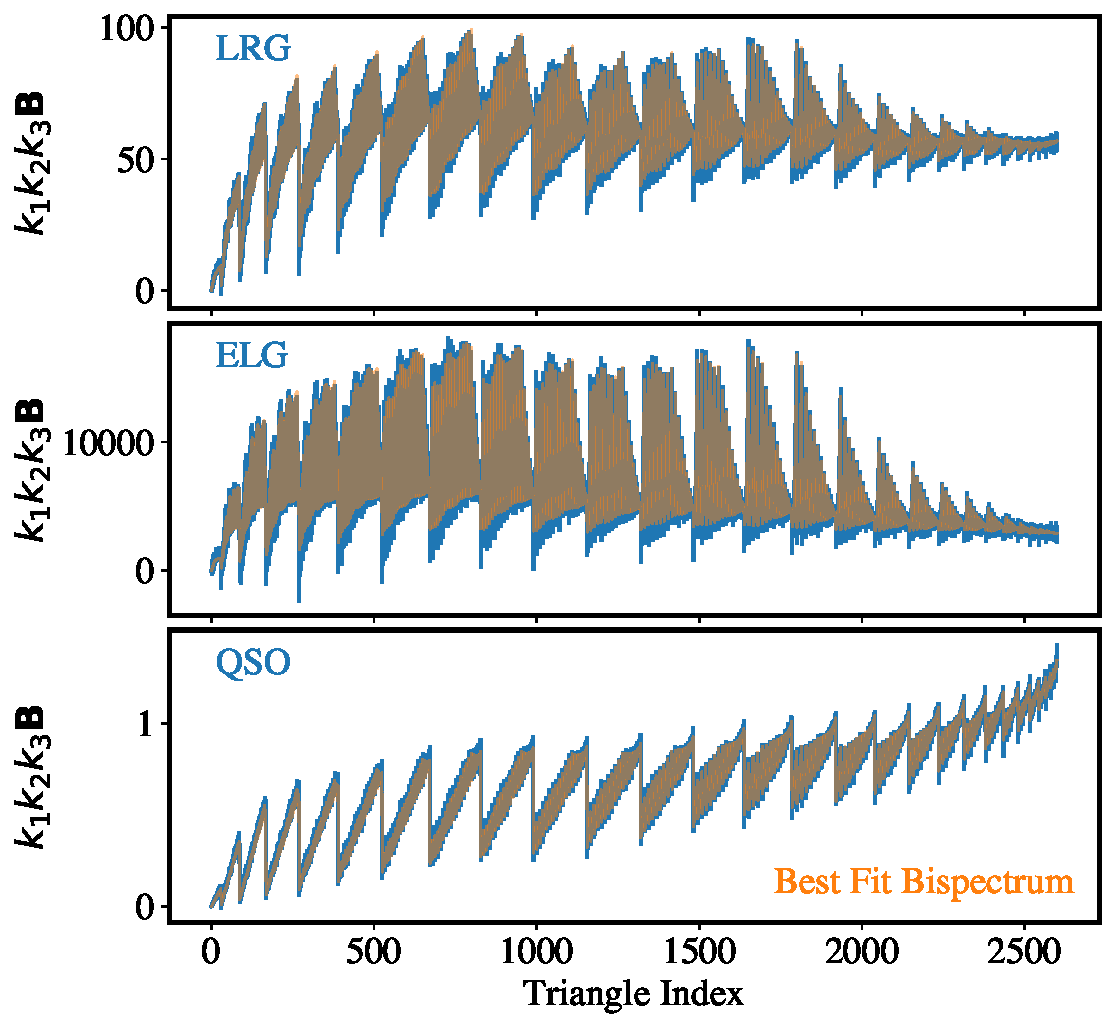
\includegraphics[width=\textwidth]{figures/spectra.pdf}
\caption{Spectra of ABACUS, GLAM, and MOLINO simulations. Top: Mean bispectrum and power spectrum of simulations relative to smooth spectrum either from the mocks (GLAM) or fitting formula (ABACUS). Bottom: Normalized dispersion of bispectrum and power spectrum.}\label{fig:data}
\end{figure*}




Scoccimarro, Couchman, and Frieman (1998): bispectrum template with plane-parallel approx and damping factor (for nonlinear effects due to velocity dispersion).



Eisenstein and Hu (1998): Power spectrum template for a general CDM-baryon universe.